\subsection{Tiles à la Google Maps}
\label{subsec:tiles}
\Gls{Maptiler} bietet auf ihrer Webseite\footnote{\url{http://www.maptiler.org/google-maps-coordinates-tile-bounds-projection/}} ein Python Script an, welches den Umgang mit Tiles stark vereinfacht. Unter anderem wird die Umrechnung von Meter zu Latitude/Longitude, Meter zu Pixel und Tiles zu QuadTree\footnote{\url{https://msdn.microsoft.com/en-us/library/bb259689.aspx}} (Bing Format für Tiles) zur Verfügung gestellt.\\

\begin{figure}[H]
\centering
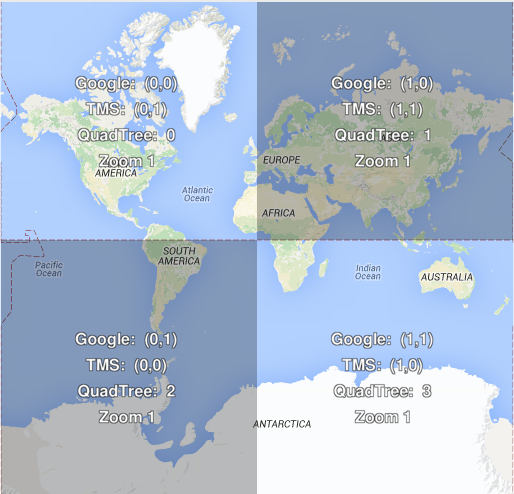
\includegraphics[width=150pt]{images/tiles_a_la_google.png}
\caption[Tiles à la Google Maps]{Tiles à la Google Maps}
\end{figure}

\subsubsection{QuadKey}
Die \Gls{Quadkeys} von Bing Maps bauen sich wie auf der Abbildung ersichtlich auf. Jedes Zoomlevel führt dazu, dass der QuadKey um eine Stelle zu nimmt. Somit kann die Anzahl der Tiles für das ensprechende Zoomlevel mit dem Zoomlevel als Exponenten zur Basis 4 angegeben werden ($4^{Zoomlevel}$).  \\
\begin{figure}[H]
\centering
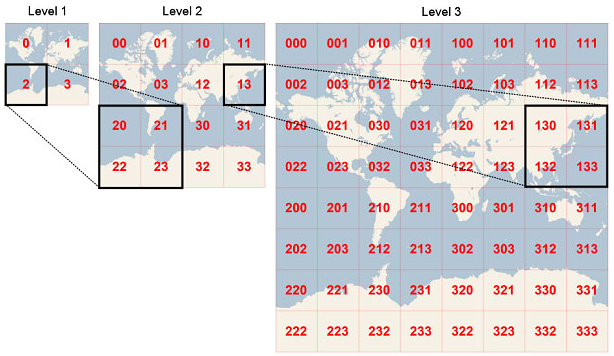
\includegraphics[width=300pt]{images/quadkey.png}
\caption[QuadTree]{QuadTree}
\end{figure}
\newpage
\subsubsection{Beispiel Code}
Das folgende Beispiel zeigt die Umrechung vom WGS84 Koordinatensystem zu Meter, zu Tiles und schlussendlich zum Quadkey. (Auf dem Zoomlevel 19) \\
\begin{python}
from src.data.globalmaptiles import GlobalMercator

zoom = 19
latitude = 47.0
longitude = 8.0
mercator = GlobalMercator()

meter_x, meter_y = mercator.LatLonToMeters(latitude, longitude)
tile_x, tile_y = self._mercator.MetersToTile(meter_x, meter_y, zoom)
quadkey = mercator.QuadTree(tile_x, tile_y, zoom)
\end{python}

